\documentclass[a4paper]{article}

\usepackage{amsmath}
\usepackage{amsfonts}
\usepackage{graphicx}
\usepackage{hyperref}
\usepackage[usenames,dvipsnames]{color}

\setlength{\parindent}{0pt}
\setlength{\parskip}{0.75ex plus 0.5ex minus 0.3ex}
\setcounter{secnumdepth}{0} % Do not number sections
\setcounter{tocdepth}{2}

\newcommand{\sympy}{\textbf{\texttt{\textcolor{OliveGreen}{SymPy}} }}

\begin{document}

\title{Linear Algebra Step by Step in \sympy}

\author{Dario Beraldi}
\maketitle
\tableofcontents

\begin{abstract}
Excerpts from \textit{Linear Algebra Step by Step} by K. Singh 
with \sympy implementation.
\end{abstract}

\section{Linear Equations and Matrices}
% =====================================

\subsection{Solving linear systems}
% ------------------------

\subsubsection{Exercises 1.1 2f} 
% ...............................................

\begin{equation}\label{eq:ex2f}
    \begin{matrix}
    e x - e y = 2 \\
    e x + e y = 0
    \end{matrix}
\end{equation}

\begin{verbatim}
x, y= symbols('x y', real= true)
eq1= Eq(E*x - E*y, 2)
eq2= Eq(E*x + E*y, 0)
sols= solve([eq1, eq2])
\end{verbatim}

Solved for:

\begin{equation}\label{eq:ex2fsol}
\begin{Bmatrix}x : e^{-1}, & y : - \frac{1}{e}\end{Bmatrix}
\end{equation}

Check solutions by substituting them in the original equations \ref{eq:ex2f}

\begin{verbatim}
eq1.subs(sols)
True
eq2.subs(sols)
True
\end{verbatim}

Solve the system \ref{eq:ex2f} using matrix notation

\begin{verbatim}
coeffs= Matrix([[E, -E], [E, E]])
const= Matrix([2, 0])
[coeffs, const]
\end{verbatim}

\begin{equation}\label{eq:}
\begin{bmatrix}\left[\begin{matrix}e & - e\\e & e\end{matrix}\right], & \left[\begin{matrix}2\\0\end{matrix}\right]\end{bmatrix}
\end{equation}

If everything is correct, solutions are consistent with \ref{eq:ex2fsol}:

\begin{verbatim}
coeffs.solve(const)
\end{verbatim}

\begin{equation}
\left[\begin{matrix}e^{-1}\\- \frac{1}{e}\end{matrix}\right]
\end{equation}

\subsubsection{Exercises 1.1 4a}
Plot the graphs of these linear equations
% .....................................................

\begin{equation}
\begin{matrix}2 x + y = 3\\x - y = 7\end{matrix}
\end{equation}

\begin{verbatim}
eq1= Eq(2*x + y, 3)
eq2= Eq(x - y, 7)
\end{verbatim}

Plot

\begin{verbatim}
pp1= plot_implicit(eq1)
pp2= plot_implicit(eq2)
pp1.extend(pp2)
pp1.save('figs/ex4a.pdf')
\end{verbatim}

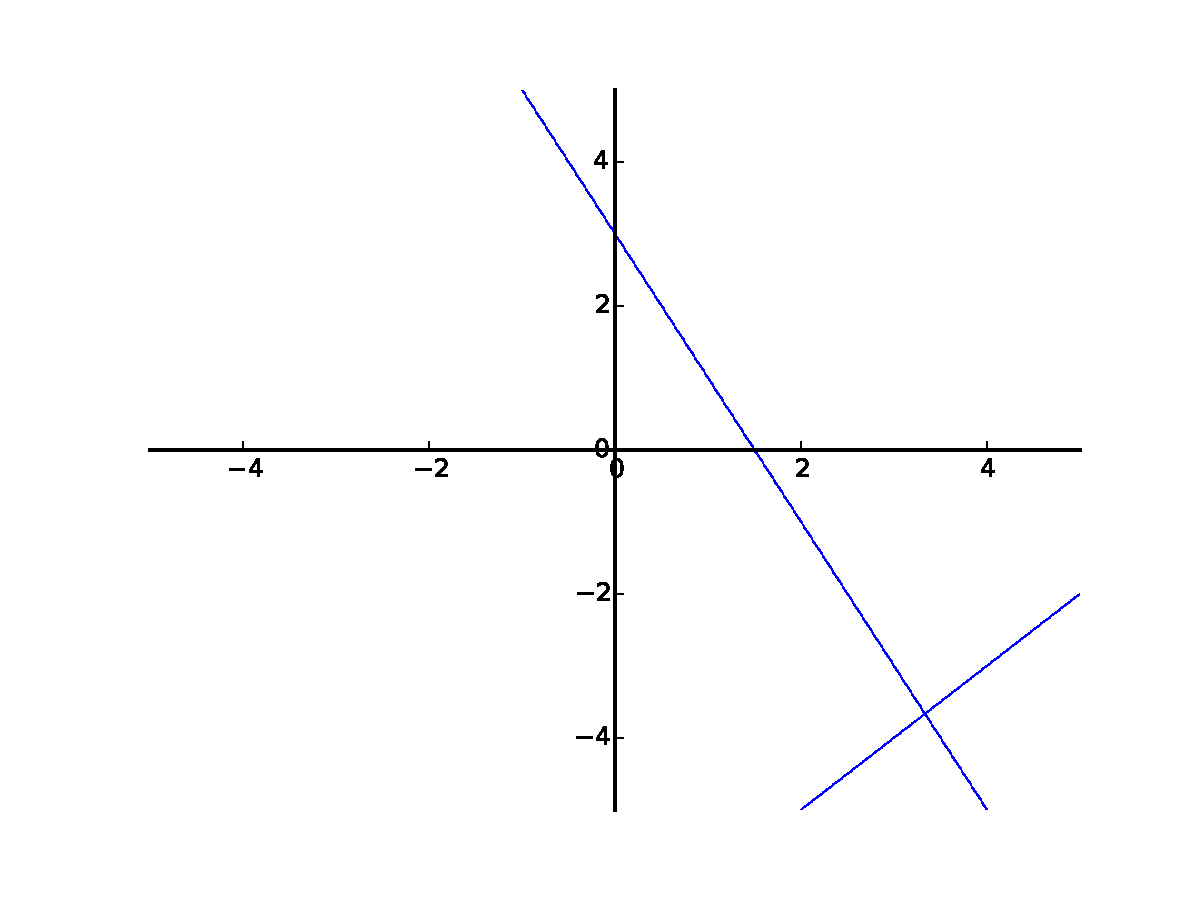
\includegraphics[width=\linewidth]{figs/ex4a.pdf}

\textbf{Exercises 1.1 5b}
% ............

\begin{verbatim}
eq1= Eq(12*x + 4*y, 16)
eq2= Eq(8*x + 4*y, 16)

pp1= plot_implicit(eq1)
pp2= plot_implicit(eq2)
pp1.extend(pp2)
pp1.save('figs/ex5b.pdf')
\end{verbatim}

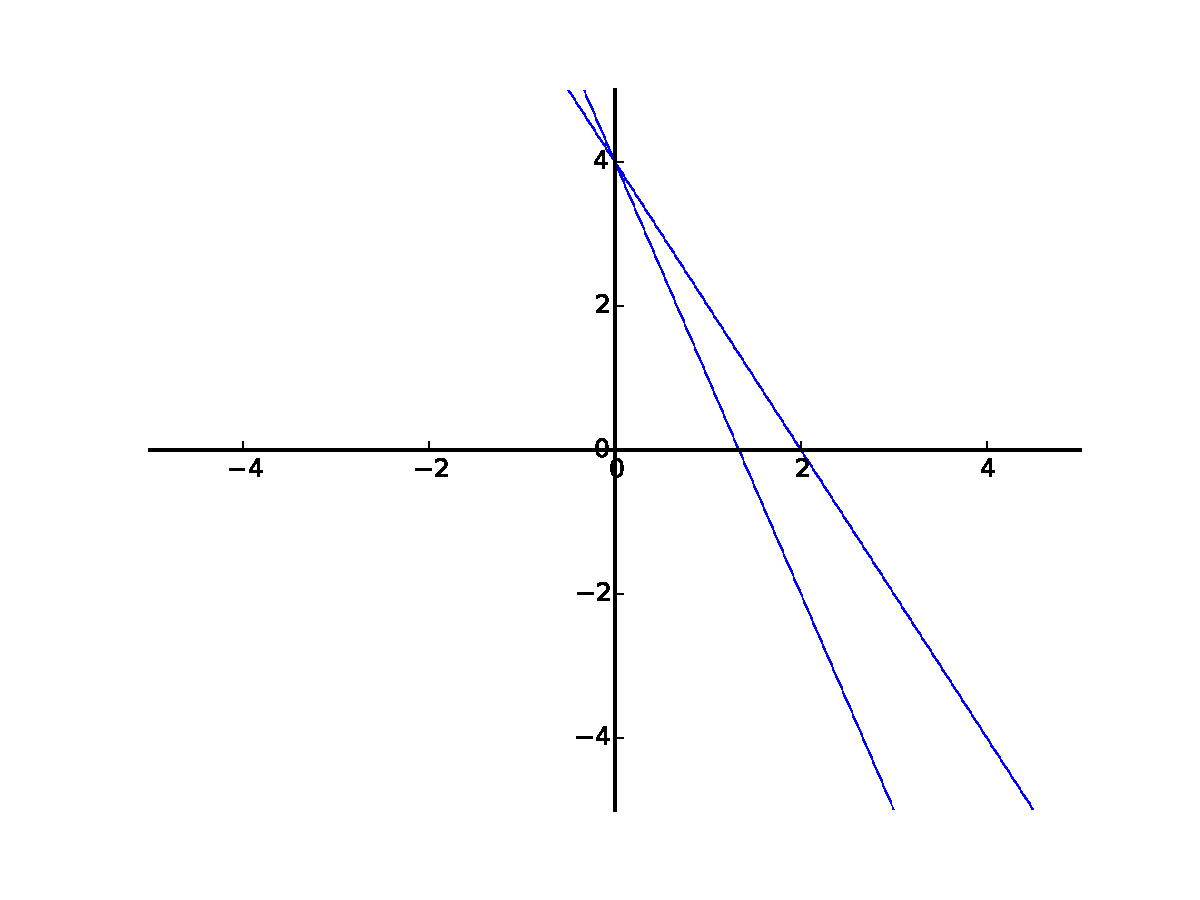
\includegraphics[width=\linewidth]{figs/ex5b.pdf}

\subsection{Solve by row echelon form}
% ------------------------------------

Given a linear system of equations, the solutions can be found by Gaussian
elimination:

\begin{itemize}
\item Extract the coefficients and constants from the equations and put them in
an augmented matrix.
\item Transform the augmented matrix in reduced row echelon form (rref). This is
the result of the Gaussian elimination process.
\item The last columns of the rref matrix lists the solutions of the linear system.
\end{itemize}

Reminder: rref means that every leading coefficient is 1 and is the only nonzero
entry in its column \footnote{http://en.wikipedia.org/wiki/Row\_echelon\_form}. 

\subsubsection{Exercises 1.2 2a}

\begin{equation}
\begin{matrix}x + 2 y + 3 z = 12\\2 x - y + 5 z = 3\\3 x + 3 y + 6 z = 21\end{matrix}
\end{equation}

\begin{verbatim}
eq1= Eq(x + 2*y + 3*z, 12)
eq2= Eq(2*x - y + 5*z, 3)
eq3= Eq(3*x + 3*y + 6*z, 21)
\end{verbatim}

Represent the linear systen as \textit{augmented} matrix, where the last column
holds the constants:

\begin{equation}
M= \left[\begin{matrix}1 & 2 & 3 & \textit{12}\\
                       2 & -1 & 5 & \textit{3}\\
                       3 & 3 & 6 & \textit{21}\end{matrix}\right]
\end{equation}

In \sympy use the \href{http://docs.sympy.org/latest/modules/polys/reference.html#sympy.polys.polytools.Poly}{\texttt{Poly}}
class to conveniently extract the coefficients at the left hand side of
the equations:

\begin{verbatim}
M= Matrix([
    Poly(eq1.lhs).coeffs(),
    Poly(eq2.lhs).coeffs(),
    Poly(eq3.lhs).coeffs()
])
const= Matrix([eq1.rhs, eq2.rhs, eq3.rhs])
M= const.col_insert(0, M)
\end{verbatim}

In reduced row echelon form, with indexes of the pivot variables on the right:

\begin{equation}
RREF= \begin{pmatrix}\left[\begin{matrix}1 & 0 & 0 & 1\\0 & 1 & 0 & 4\\0 & 0 & 1 & 1\end{matrix}\right], & \begin{bmatrix}0, & 1, & 2\end{bmatrix}\end{pmatrix}
\end{equation}

Solutions can be read from last column of the RREF $\left[\begin{matrix}x:1\\y:4\\z:1\end{matrix}\right]$. Verify the solutions solve
the initial system of equations:

\begin{verbatim}
rref= M.rref()
sols= rref[0].col(-1)

eq1.subs({x:sols[0], y:sols[1], z:sols[2]}) # True
eq2.subs({x:sols[0], y:sols[1], z:sols[2]}) # True
eq3.subs({x:sols[0], y:sols[1], z:sols[2]}) # True

# Or the same returning dict {x: 1, y: 4, z: 1}
solve([eq1, eq2, eq3]) 
\end{verbatim}

\subsubsection{Exercises 1.2 3d}
% ..............................

Linear system:

\begin{equation}
\begin{matrix}
    - 2 x + 3 y - 2 z = 8 \\
    - x + 2 y - 10 z = 0 \\
    5 x - 7 y + 4 z = -20
\end{matrix}
\end{equation}

Augmented matrix:

\begin{equation}
\left[\begin{matrix}-2 & 3 & -2 & 8\\-1 & 2 & -10 & 0\\5 & -7 & 4 & -20\end{matrix}\right]
\end{equation}

Reduced row echelon form with solutions in the last column:

\begin{equation}
\begin{pmatrix}\left[\begin{matrix}1 & 0 & 0 & -3 \\
                                   0 & 1 & 0 & 1 \\
                                   0 & 0 & 1 &
\frac{1}{2}\end{matrix}\right], & \begin{bmatrix}0, & 1, & 2\end{bmatrix}\end{pmatrix}
\end{equation}

In \sympy:

\begin{verbatim}
eq1= Eq(-2*x + 3*y -2*z, 8)
eq2= Eq(-x + 2*y - 10*z, 0)
eq3= Eq(5*x - 7*y + 4*z, -20)

M= Matrix([
    Poly(eq1.lhs).coeffs(),
    Poly(eq2.lhs).coeffs(),
    Poly(eq3.lhs).coeffs()
])
const= Matrix([eq1.rhs, eq2.rhs, eq3.rhs])
M= const.col_insert(0, M)
rref= M.rref()
sols= rref[0].col(-1)

# Checked: {x: -3, y: 1, z: 1/2}
solve([eq1, eq2, eq3])
\end{verbatim}

\subsection{Vector arithmetic}
% ----------------------------

\subsubsection{Exercise 1.3.1}

Given two vectors:

\begin{verbatim}
va= Matrix([2, 0])
vb= Matrix([2, 1])

fig = plt.figure()
fig.add_subplot(111)

\end{verbatim}

plot the results of the operations 

\subsubsection{(a-e)}

\begin{verbatim}
vA= va + vb          # [4 1]
vB= va - vb          # [0 -1]
vC= 3 * va           # [6 0]
vD= -1/2 * vb        # [-1 -0.5]
vE= 3*va - 1/2 * vb  # [5 -0.5]
\end{verbatim}

And plot vectors

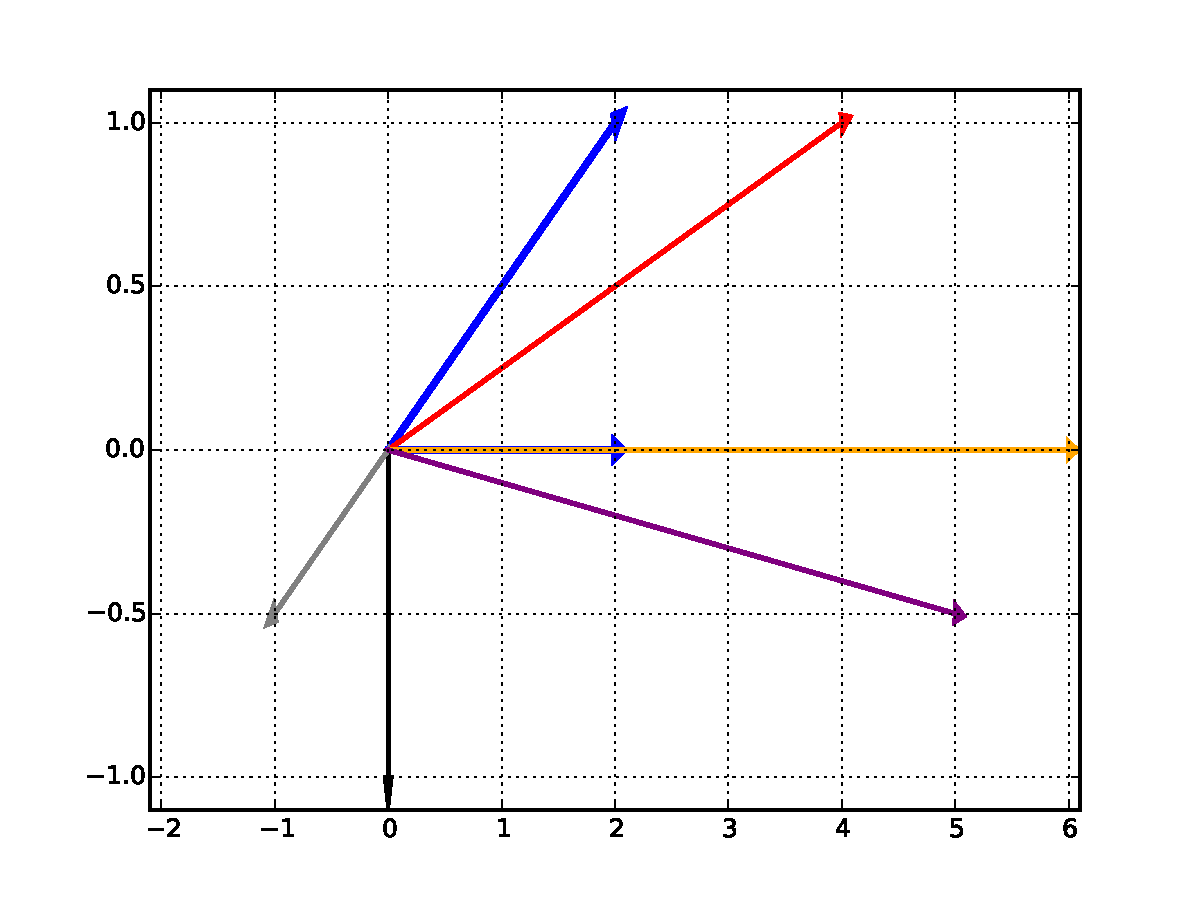
\includegraphics[width=\linewidth]{figs/ex1_3.pdf}

\begin{verbatim}
plt.arrow(0, 0, float(va[0]), float(va[1]), lw= 3, color= 'b', head_width=0.05)
plt.arrow(0, 0, float(vb[0]), float(vb[1]), lw= 3, color= 'b', head_width=0.05)
plt.arrow(0, 0, float(vA[0]), float(vA[1]), lw= 2, color= 'r', head_width=0.05)
plt.arrow(0, 0, float(vB[0]), float(vB[1]), lw= 2, color= 'black', head_width=0.05)
plt.arrow(0, 0, float(vC[0]), float(vC[1]), lw= 2, color= 'orange', head_width=0.05)
plt.arrow(0, 0, float(vD[0]), float(vD[1]), lw= 2, color= 'grey', head_width=0.05)
plt.arrow(0, 0, float(vE[0]), float(vE[1]), lw= 2, color= 'purple', head_width=0.05)
plt.xlim(-2.1, 6.1)
plt.ylim(-1.1, 1.1)
plt.grid()
plt.savefig('figs/ex1_3.pdf')
plt.close()
\end{verbatim}

\subsubsection{Exercise 1.3.8}
% ............................
Show that $x\mathbf{u} + y\mathbf{v} = \mathbf{w}$ where
$\mathbf{u}= (1\ 0)^{T}$, $\mathbf{v}= (0\ 1)^{T}$, and $\mathbf{w}= (x\ y)^{T}$.

This is a consequence of $x(1\ 0) = (x\ 0)$ and $y(0\ 1) = (y\ 0)$. So that
$(x\ 0) + (0\ y) = (x\ y)$

\begin{verbatim}
x, y= symbols('x y')
u= Matrix([1, 0])
v= Matrix([0, 1])
w= Matrix([x, y])
Eq(x*u + y*v, w) # True
\end{verbatim}

\subsubsection{Exercise 1.3.12}
% .............................

Find the real numbers x, y and z, if

\begin{equation}
\left[\begin{matrix}x - 2 z\\2 x + y\\- y + 6 z\end{matrix}\right] = \left[\begin{matrix}5\\3\\17\end{matrix}\right]
\end{equation}

Which is solved for:

\begin{equation}
sols= \begin{bmatrix}\begin{Bmatrix}x : 7, & y : -11, & z : 1\end{Bmatrix}\end{bmatrix}
\end{equation}

\begin{verbatim}
eq1= Eq(x * Matrix([1, 2, 0]) + y * Matrix([0, 1, -1]) + z * Matrix([-2, 0, 6]),
    Matrix([5, 3, 17]))
sols= solve(eq1)
\end{verbatim}

\subsubsection{Exercise 1.3.12}
% .............................

Show that vectors \textbf{u} and \textbf{v} in space $\mathbb{R}^n$ can be
$\mathbf{u} \cdot{} \mathbf{v} = \mathbf{0}$ even if neither \textbf{u} or \textbf{v}
are 0 vectors.

Set:

\begin{verbatim}
u= Matrix([-1, 1])
v= Matrix([1, 1])
u.dot(v) == 0 # True
\end{verbatim}

\subsection{Linear equations and Matrices}
% ----------------------------------------


%%%%%%%%%%%%%%
\end{document}
